
% Template for Elsevier CRC journal article
% version 1.0 dated 13 October 2009

% This file (c) 2009 Elsevier Ltd.  Modifications may be freely made,
% provided the edited file is saved under a different name

% This file contains modifications for Procedia Computer Science

%%%%%%%%%%%%%%%%%%%%%%%%%%%%%%%%%%%%%%%%%%%%%%%%%%%%%%%%%%%%%%%%%%%%%%%%%%

%% This template uses the elsarticle.cls document class and the extension package ecrc.sty
%% For full documentation on usage of elsarticle.cls, consult the documentation "elsdoc.pdf"
%% Further resources available at http://www.elsevier.com/latex

%%%%%%%%%%%%%%%%%%%%%%%%%%%%%%%%%%%%%%%%%%%%%%%%%%%%%%%%%%%%%%%%%%%%%%%%%%

%% The '3p' and 'times' class options of elsarticle are used for Elsevier CRC
\documentclass[3p,times]{elsarticle}

%% The `ecrc' package must be called to make the CRC functionality available
\usepackage{ecrc}

%% The ecrc package defines commands needed for running heads and logos.
%% For running heads, you can set the journal name, the volume, the starting page and the authors

%% set the volume if you know. Otherwise `00'
\volume{00}

%% set the starting page if not 1
\firstpage{1}

%% Give the name of the journal
\journalname{Procedia Computer Science}

%% Give the author list to appear in the running head
%% Example \runauth{C.V. Radhakrishnan et al.}
\runauth{}

%% The choice of journal logo is determined by the \jid and \jnltitlelogo commands.
%% A user-supplied logo with the name <\jid>logo.pdf will be inserted if present.
%% e.g. if \jid{yspmi} the system will look for a file yspmilogo.pdf
%% Otherwise the content of \jnltitlelogo will be set between horizontal lines as a default logo

%% Give the abbreviation of the Journal.
\jid{procs}

%% Give a short journal name for the dummy logo (if needed)
\jnltitlelogo{Procedia Computer Science}

%% Hereafter the template follows `elsarticle'.
%% For more details see the existing template files elsarticle-template-harv.tex and elsarticle-template-num.tex.

%% Elsevier CRC generally uses a numbered reference style
%% For this, the conventions of elsarticle-template-num.tex should be followed (included below)
%% If using BibTeX, use the style file elsarticle-num.bst

%% End of ecrc-specific commands
%%%%%%%%%%%%%%%%%%%%%%%%%%%%%%%%%%%%%%%%%%%%%%%%%%%%%%%%%%%%%%%%%%%%%%%%%%

%% The amssymb package provides various useful mathematical symbols
\usepackage{amssymb}
%% The amsthm package provides extended theorem environments
%% \usepackage{amsthm}

%% The lineno packages adds line numbers. Start line numbering with
%% \begin{linenumbers}, end it with \end{linenumbers}. Or switch it on
%% for the whole article with \linenumbers after \end{frontmatter}.
%% \usepackage{lineno}

%% natbib.sty is loaded by default. However, natbib options can be
%% provided with \biboptions{...} command. Following options are
%% valid:

%%   round  -  round parentheses are used (default)
%%   square -  square brackets are used   [option]
%%   curly  -  curly braces are used      {option}
%%   angle  -  angle brackets are used    <option>
%%   semicolon  -  multiple citations separated by semi-colon
%%   colon  - same as semicolon, an earlier confusion
%%   comma  -  separated by comma
%%   numbers-  selects numerical citations
%%   super  -  numerical citations as superscripts
%%   sort   -  sorts multiple citations according to order in ref. list
%%   sort&compress   -  like sort, but also compresses numerical citations
%%   compress - compresses without sorting
%%
%% \biboptions{comma,round}

% \biboptions{}

% if you have landscape tables
\usepackage[figuresright]{rotating}

% put your own definitions here:
%   \newcommand{\cZ}{\cal{Z}}
%   \newtheorem{def}{Definition}[section]
%   ...

% add words to TeX's hyphenation exception list
%\hyphenation{author another created financial paper re-commend-ed Post-Script}

\providecommand{\e}[1]{\ensuremath{\times 10^{#1}}}
\usepackage[normalem]{ulem}
\usepackage{algorithmic}
\usepackage{epsfig}
% declarations for front matter

\begin{document}

\begin{frontmatter}

%% Title, authors and addresses

%% use the tnoteref command within \title for footnotes;
%% use the tnotetext command for the associated footnote;
%% use the fnref command within \author or \address for footnotes;
%% use the fntext command for the associated footnote;
%% use the corref command within \author for corresponding author footnotes;
%% use the cortext command for the associated footnote;
%% use the ead command for the email address,
%% and the form \ead[url] for the home page:
%%
%% \title{Title\tnoteref{label1}}
%% \tnotetext[label1]{}
%% \author{Name\corref{cor1}\fnref{label2}}
%% \ead{email address}
%% \ead[url]{home page}
%% \fntext[label2]{}
%% \cortext[cor1]{}
%% \address{Address\fnref{label3}}
%% \fntext[label3]{}

\dochead{International Conference on Computational Science, ICCS 2012}
%% Use \dochead if there is an article header, e.g. \dochead{Short communication}

\title{Towards speed up search of maximal unique matches in multicore architectures}

%% use optional labels to link authors explicitly to addresses:
%% \author[label1,label2]{<author name>}
%% \address[label1]{<address>}
%% \address[label2]{<address>}

\author{}

\address{}

\begin{abstract}
  Maximal Unique Matches are common substrings that are found between a reference and a query sequence. They are exact, unique and maximal; that is, they cannot be extended in left or right direction without incurring a mismatch. The computation of MUMs in large sequences is a heavy and repetitive task because the genomes are closely related, so there is a fair chance of parallelize and execute this search in multicore architectures. This research resembles a first novel approach to find MUMs in genomic sequences in parallel way. The reference genome is indexed by using a suffix tree in main memory and then the parallelized algorithm finds the MUMs against a query genome which is readed by several threads. This approach is based on MUMmer, a genome alignment tool, which is able to find Maximal Unique Matches (MUMs). 
\end{abstract}

\begin{keyword}
%% keywords here, in the form: keyword \sep keyword

%% PACS codes here, in the form: \PACS code \sep code

%% MSC codes here, in the form: \MSC code \sep code
%% or \MSC[2008] code \sep code (2000 is the default)

\end{keyword}

\end{frontmatter}

%%
%% Start line numbering here if you want
%%
% \linenumbers

%% main text
\section{Problem}
\label{}
The problem of searching maximal unique matching for a minimum lengthbetween a reference
string and a query string has been
identified in several applications, one of them is MUMmer. Altough
MUMmer's algorithm can perform searches of maximal unique matches (MUMs)
the use of resources are not well used:
\begin{itemize}
  \item High use of main memory to store the reference string.
  \item A null use of multicore architectures.
\end{itemize}
If the length of reference and query are very huge, the amount of operations to perform
in the search of MUMs increases, see table \ref{tbl:operations}.
\begin{table}[ h!]
  \begin{small}
    \begin{center}
      \begin{tabular}{lllll}
        Data structure & L [bp\footnote{Base pair, basic measure unit of nucleotides for a DNA sequence.}] & Search  & Search [s] & Memory\\
        & & operations & & usage [MB]\\
        \hline
        Suffix tree & 20 & 9,87\e{18}  & 169189,4 & 48665,12\\
        \hline
      \end{tabular}
    \end{center}
  \end{small}
  \caption{Search of Maximal Unique Matches between a reference sequence (2960,21Mbp) and query sequence (2716,96Mbp)}
  \label{tbl:operations}
\end{table}
The use of parallelism could help reduce the execution time for the search of maximal unique matches. One approach of
parallelism is to take advantage of multicore architectures nowadays.\\
This problem has a time complexity of $O(m+k)$ where $m$ is the length of the query sequence and $k$ is the number of 
maximal unique matches of some minimum length. This problem is a very high intensive computing task, for every substring
in the query sequence the search for a maximum unique match has to be performed.\\
\section{The MUM: an heuristic approach}
\subsection{Definition MUM}
Although a pair of conserved genes rarely contain the same entire sequence, they share a lot of short common substrings and some of them are indeed unique to this pair of genes. For example the following two sequences, R and Q:\\
\begin{center}
    R=\underline{ac} ga \underline{ctc} a \underline{gctac} t \underline{ggtcagctatt} \underline{acttaccgc}\$\\
      Q=\underline{ac} tt \underline{ctc} t \underline{gctac} \underline{ggtcagctatt} c \underline{acttaccgc}\$\\
    \end{center}
    It is clear that sequences R and Q have many common substrings, they are:
    \begin{itemize}
      \item ac
      \item ctc
      \item gctac
      \item ggtcagctatt
      \item acttaccgc
    \end{itemize}
Among those five common substrings, ac is the only substring that is not unique. It occurs more than once in both sequences. You can also observe that actually a, c, t, and g are common substrings of R and Q. However, they are not maximal, i.e. they are contained in at least one longer common substrings. We are only interested in those that are of maximal length.\\
Our aim is to search for all these short common substrings. Given genomes R and Q, we need to find all common substrings which are unique and of maximal length. Each of such common substrings is known as Maximum Unique Match (MUM). For almost every conserved gene pairs, there exist at least one MUM which is unique to them.\\
For example, assuming d = 3, sequences R and Q in the previous example has four MUMs: ctc, gctac, ggtcagctatt, acttaccgc. Substring ac is not an MUM because its length is smaller than the value of d and it is not unique to both sequences.
\begin{center}
    R=\xout{ac} ga \sout{ctc} a \uwave{gctac} t \uuline{ggtcagctatt} \uline{acttaccgc}\$\\
      Q=\xout{ac} tt \sout{ctc} t \uwave{gctac} \uuline{ggtcagctatt} c \uline{acttaccgc}\$\\
    \end{center}
The concept of MUM is important in whole genome alignment because a significantly long MUM is very likely to be part of the global alignment.
\subsubsection{Finding MUMs in a suffix tree} 
The key idea in this method is to build a suffix tree for genome R, a data structure which allows finding, extremely efficiently, all distinct subsequences in a given sequence.\\
  By construction, the location of a match in the suffix tree represents a substring of the subject sequence which maximaly matches a prefix of
  \texttt{query suffix}. Thus it is only necessary to verify that, the substring of the subject sequence is long enough, that it is unique in the subject sequence and that 
  the match is also left maximal. This is done as follows:
  
  \begin{enumerate}
  \item
  Does \texttt{location} represent a substring of length at least \texttt{minimum match length}?
  \item 
  Does \texttt{location} correspond to a leaf edge? Then then the string represented by the location is unique in the subject sequence.
  \item 
  Is the substring left maximal? This is true if one of the following conditions hold:
  \begin{itemize}
  \item 
  The suffix of the query currently considered is the first suffix, or 
  \item
  The string represented by \texttt{loc} is a prefix of the subject string,  or
  \item 
  The characters immediately to the left of the matching strings in the subject sequence and the query sequence are different
  \end{itemize}
  \end{enumerate}
  If all conditions 1-3 are true, then this MUM is stored in a list of MUM-candidates, see Figure \ref{candidates}. 
 \begin{figure}[htb]  
 \begin{center} 
  \includegraphics[width=6.5cm,height=4cm]{MUM-candidates.png}
 \end{center} 
 \caption{Finding MUMs in a suffix tree.} 
 \label{candidates} 
 \end{figure}  
  It takes the necessary information about the MUM-candidate:
  \begin{itemize}
    \item Position in reference sequence.
    \item Position in query genome.
    \item Length of match.
  \end{itemize}
MUMs can cover 100\% of the known  conserved gene pairs. Moreover, finding all MUMs can be done in almost linear time.
\section{Parallelism technique}  
General-purpose, commodity CPUs currently have SIMD (Single Instruction Multiple Data) functional units and corresponding SIMD instructions. This kind of CPUs allow to be used in several ways of parallel techniques, such as data-level parallelism. \\
In addition to using SIMD technology, the availability of multicore architecture makes possible to execute the same task with a different kind of data.\\
The sequential version of the MUMmer's algorithm trades extra computation for memory and high computation time when executed in a single machine. \\
Previously the algorithm for sequence alignment was described in detail. Now our own proposal of a parallelization of WGA within multicore architecture is explained. There are two resources to improve in this algorithm:
\begin{itemize}
\item Memory usage.
\item Running time.
\end{itemize}
The former was generally improved because it allows being executed in architecures where there is no restriction memory. To improve the performance of the algorithm a data-level parallelism technique is deployed in advance to genome alignment.\\
Our technique is divided in three phases following:
\begin{enumerate}
\item Splitting genome data (chunks) according to the number of available cores using 1 thread per core.
\item Parallel execution of the task of finding MUMs for every chunk where every thread has its own list of MUM-candidate.
\item Get the final list of MUMs from every MUM-candidate list of all threads.
\end{enumerate}
The following Figure \ref{algorithm} shows the process of our data-level parallelism technique.
\begin{figure}[htb]  
\begin{center} 
  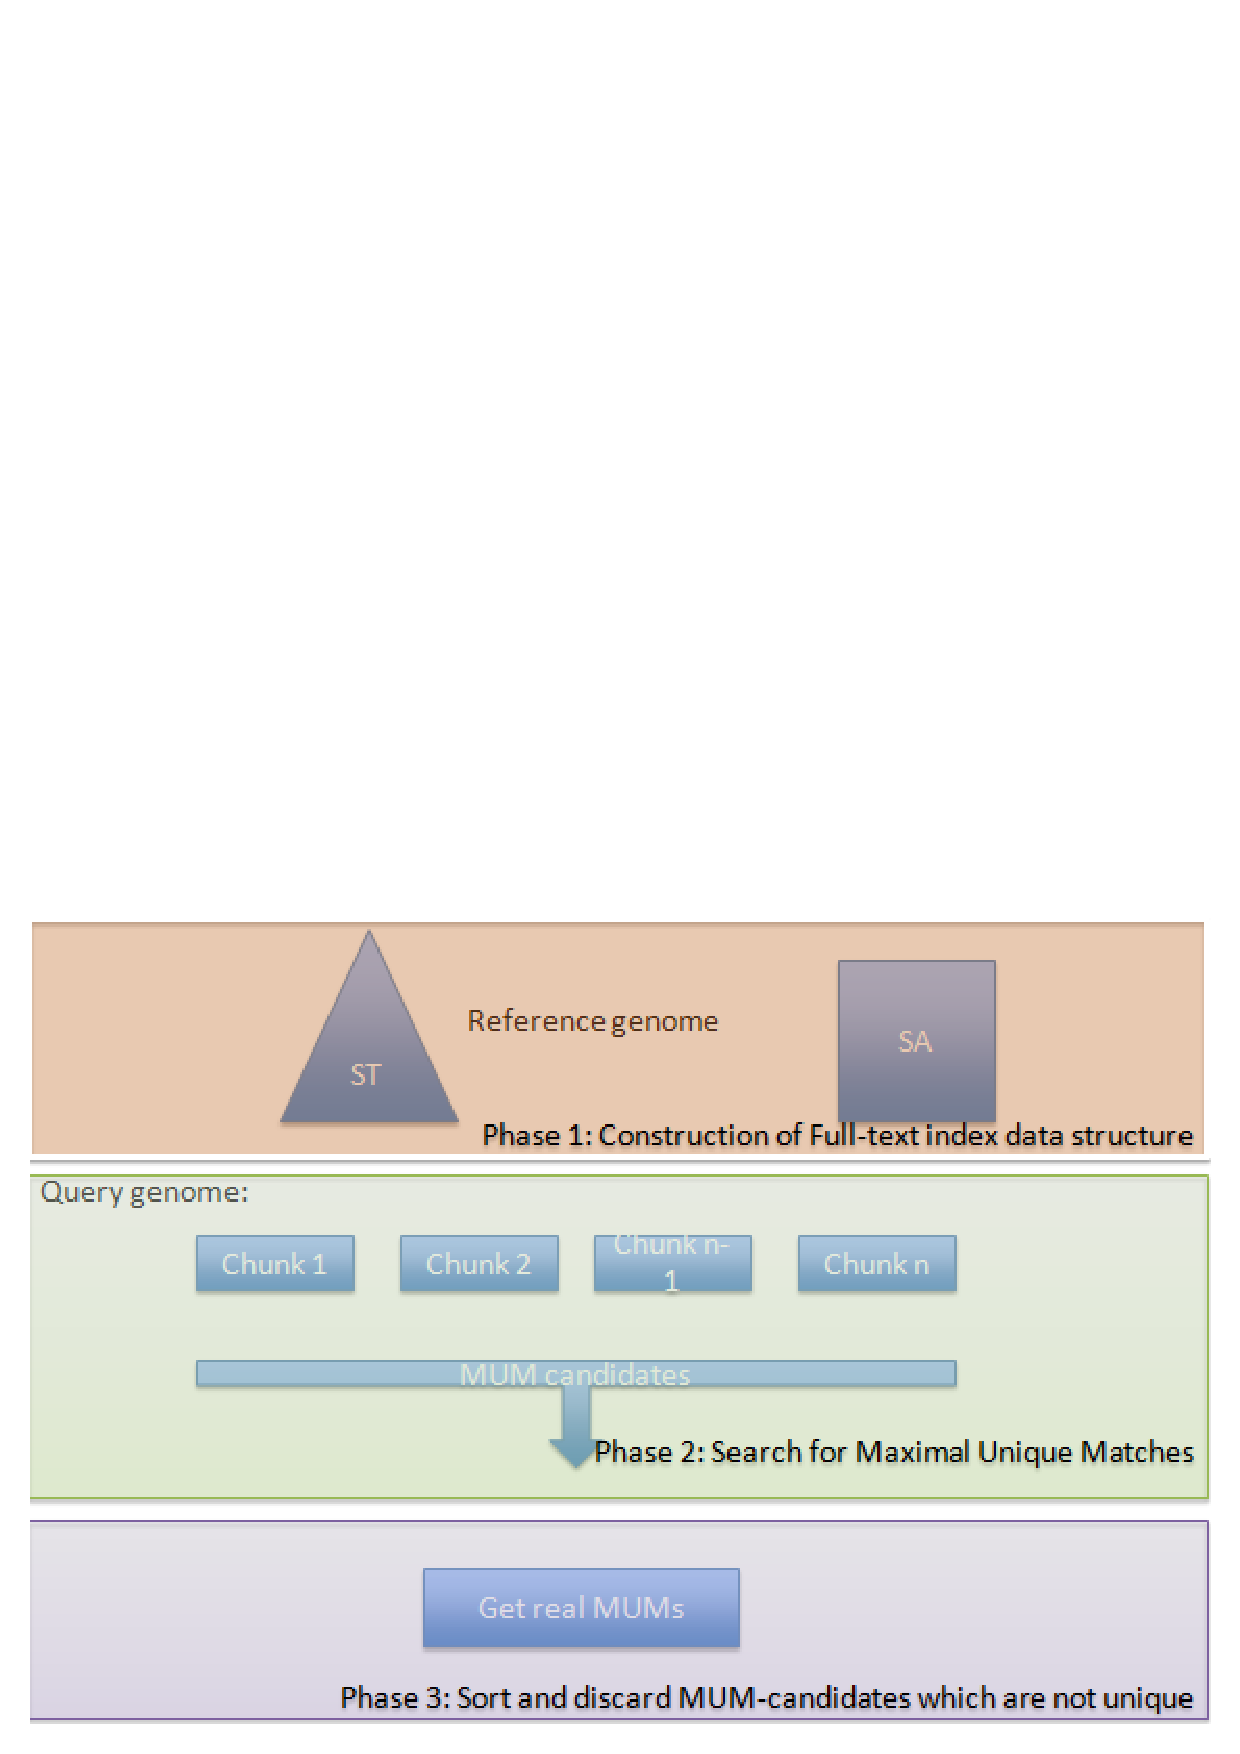
\includegraphics[width=4.5cm,height=4cm]{Phases.png}
\end{center} 
\caption{Data-level parallelism in multicore architectures for whole genome alignment.} 
\label{algorithm} 
\end{figure} 
The division of genome data was used using the paradigm of data-level parallelism which consists of a generation of chunks of a query sequence with a fixed size. 
The main idea behind using a Maximal Unique Match (MUM): it is possible to cover a huge region of a genome when reference and query genomes are very closely related. However 
to get a MUM, it requires an important feature its uniqueness. 
%We had to face with concept while we evaluated different ways to implement the data-level parallelism. 
Uniqueness can only be found when a whole genome is checked, see Figure \ref{Whole-MUM}. If some part of it is only evaluated we could miss the rest of the genome. In other words, after finding MUMs within a chunk it is not possible to determine if the MUM found is or not a "unique" MUM, globally in the query genome,  because these MUMs are unique only in the chunk that has been read, the rest of the genome it is not known until all query genome has been read, see Figure \ref{Whole-MUM}.\\
\begin{figure}[htb]  
\begin{center} 
  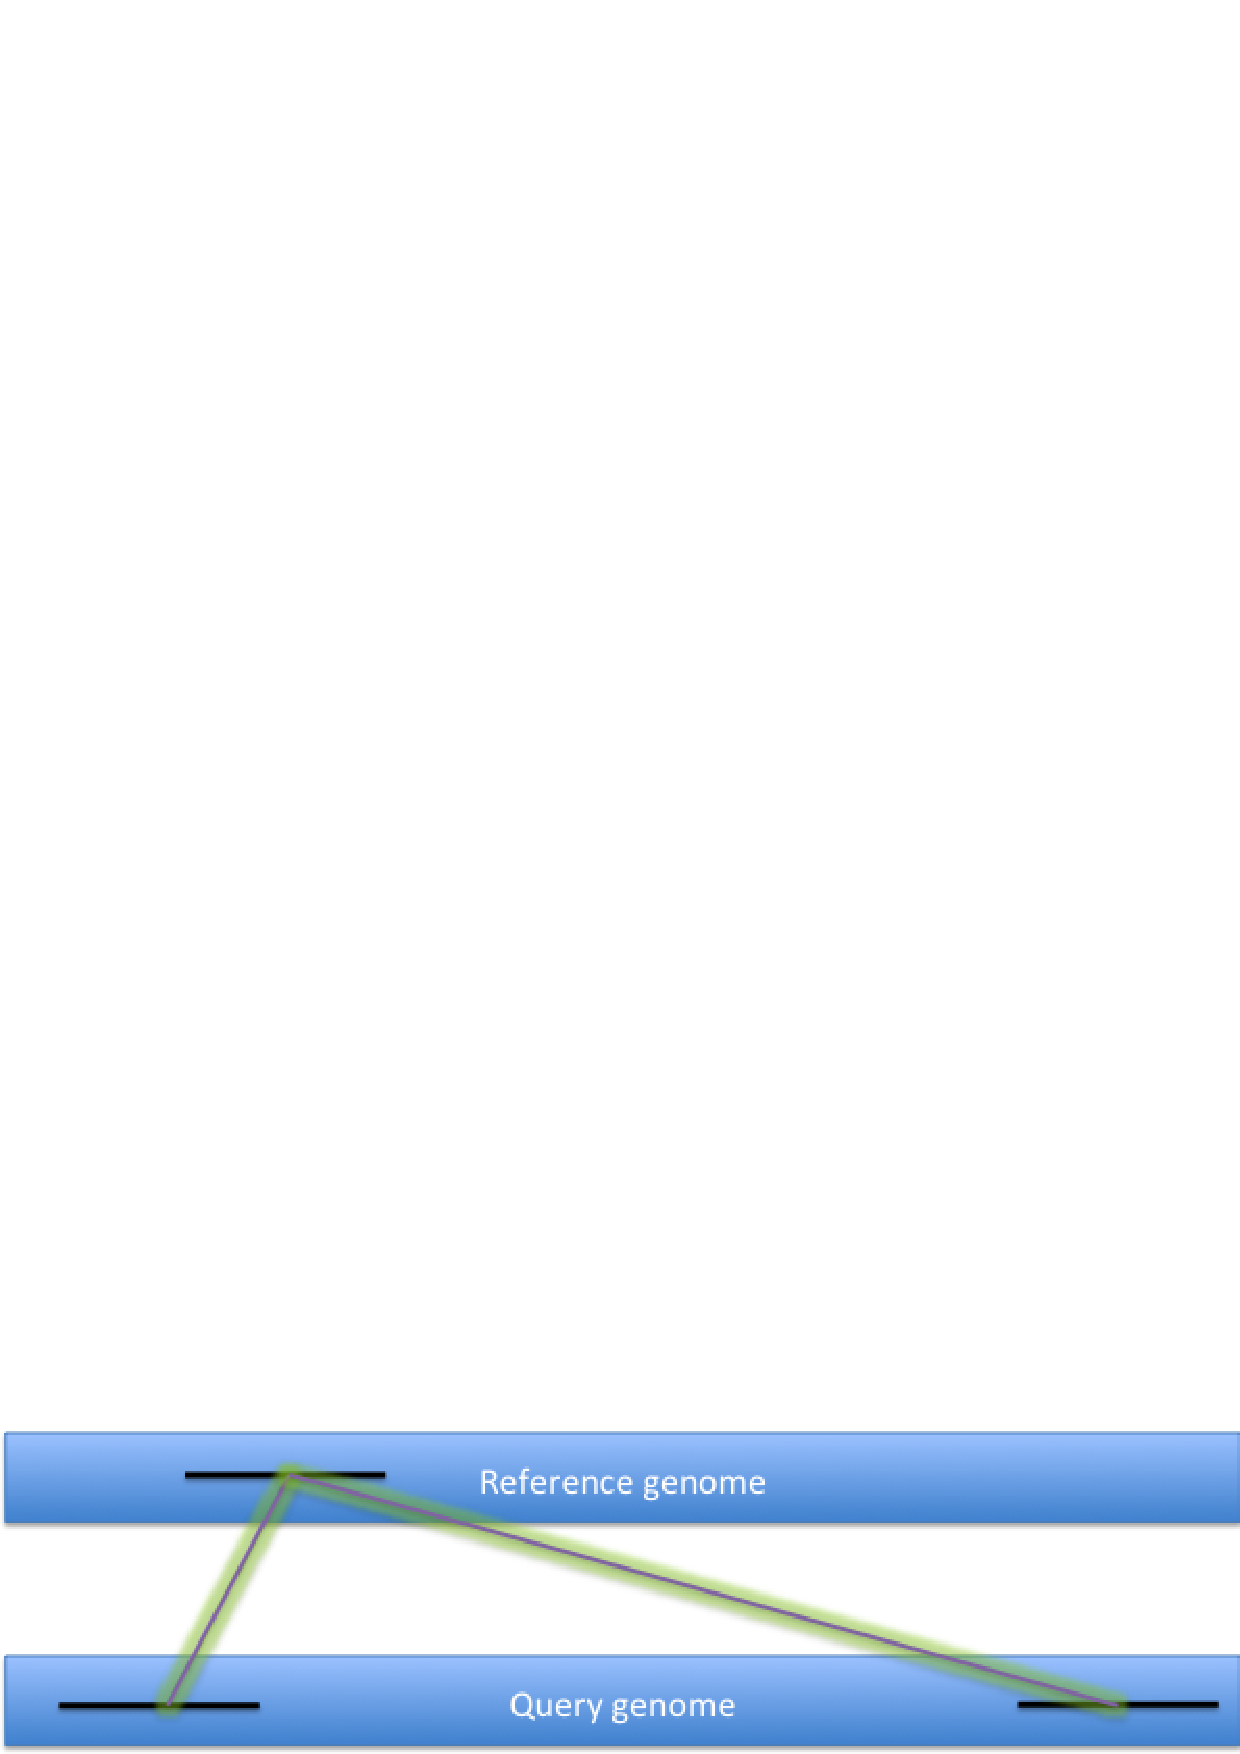
\includegraphics[width=6cm,height=3cm]{Whole-MUM.png}
\end{center} 
\caption{MUM in reference genome but not in query genome.} 
\label{Whole-MUM} 
\end{figure}
\section{Implementation} 
\label{implementation}
\subsection*{Split query genome}  
As it was previously explained, the approach is to use a fixed size division of query genome in as many chunks as  many available cores. 
To split query genome the algorithm needs to know in advance how many chunks will be used. Then every chunk is computed with two pointers (left and right end)
which points out query genome in main memory.
\subsection*{Finding MUMs}
The parallelization is carried out with OpenMP. The algorithm to find MUMs is a process which can be executed without any data dependency. However, when we split a query sequence the following problems arise:
\begin{itemize}
  \item Chunk size is a performance factor.
  \item Different MUM-candidate in query sequence:
    \begin{itemize}
      \item Additional MUMs.
      \item Lost MUMs.
    \end{itemize}
\end{itemize}
OpenMP defines the schedule for the loop iterations among the total number of threads. The total number of iterations is the number of chunks created. Every iteration means the whole search of MUMs within a chunk, if the right end of chunk is not the end of the query sequence and there are still nucleotides to match then traversal of suffix tree until it occurs a mismatch or a MUM-candidate is found.\\
The key factors in this phase are:
\begin{itemize}
  \item Number of chunks.
  \item Size of chunks.
  \item Number of threads.
  \item OpenMP schedule and its own chunk size.
\end{itemize}
\subsection*{Get real MUMs}
List of MUM-candidates are ordered with quicksort according to position in query sequence. Every thread has found a set of MUM-candidates from previous phase but the all threads don't produce the MUM-candidates in order. That's why a quicksort is required.\\
After quicksort we need to get the real MUMs. A real MUM is unique in the whole reference and query genome. Those MUM-candidates which are overlapped by bigger MUMs are discarded, see Figure \ref{real-mums}.\\
\begin{figure}[htb]  
\begin{center} 
  \includegraphics[width=4.5cm,height=4cm]{MUMs.png}
  \includegraphics[width=4.5cm,height=4cm]{Remove-MUMs.png}
\end{center} 
\caption{Getting Real MUMs.} 
\label{real-mums} 
\end{figure}
The final output has the following format:
\begin{verbatim} 
>Information about the query sequence
Position_in_R Position_in_Q Length_of_MUM
\end{verbatim}
\section{Experiments and results}
To verify that our approach, can have a better performance to align a whole genome a set of tests were deployed. These tests were carried out in the following node:
\begin{itemize}
\item Hardware:  
\begin{itemize}
\item 2 Processor Intel(R) Xeon(R) E5645 @ 2.4GHz of 6 cores each one, 32KB L1 cache, 256KB L2 and 12MB L3 shared cache per socket.
\item RAM: 96 GB
\end{itemize}
\item  Software: 
\begin{itemize}
\item Linux Kernel 2.6.32-220.el6.x86\_64 \#1 SMP
\item gcc 4.7.0 with OpenMP support
\item Likwid 2.3.0
\end{itemize}
\item Genomes:
  \begin{itemize}
    \item Reference: Human chromosome 21 single fasta file
    \item Query: Mouse chromosome 16 single fasta file
  \end{itemize}
\end{itemize}
The main objective of the tests was check the performance of finding MUMs in multicore architectures by using OpenMP (threads). The variables to control were:
\begin{enumerate}
  \item Number of chunks.
  \item Number of threads.
\end{enumerate}

%% \appendix

%% \section{}
%% \label{}

%% References
%%
%% Following citation commands can be used in the body text:
%% Usage of \cite is as follows:
%%   \cite{key}         ==>>  [#]
%%   \cite[chap. 2]{key} ==>> [#, chap. 2]
%%

%% References with BibTeX database:
\section*{References}
\bibliographystyle{elsarticle-num}
\bibliography{mum-multithread}

\end{document}

%%
%% End of file `procs-template.tex'. 
